\section{本実験}
予備実験より上がった問題点をまとめたものを以下に簡潔にまとめる.
・香りの量,濃度が不十分
・香料の出し方の増強を検討
・ゼリーの大きさの変更
・無味のゼリーへの不快感の改善
これらの課題点を踏まえた上で新たに構築したシステムと実験方法について述べていく.


\subsection{風味変容システムの概要}

嗅覚情報を風味として付与する仕組みとして,予備実験を踏まえたうえで Vape のリキッドを
使用して気化させた香料を中に閉じこめる風味強化した新たなシステムを試作している.予備実
験のバニラの香りと醤油の香りの他にワインを気化した香りを空洞のゼリーに入れて食したとこ
ろ,アルコールとワインの香りをバニラと醤油の二種類よりも強く感じた.そのため,アルコー
ルのような気化しやすい液体を混ぜて中に入れゼリーの中で気化して充満させることでより香料
の濃度を上がることが出来ると考えた.


そこで,香料を気化して吸うことで様々な味を味わうことができる Vape の香料の素であるリ
キッドを利用することであり,予備実験で使用していた香料よりも香りの量,濃度を上げること
を可能とする.


これらによって,予備実験で上がった香りの量,濃度が不十分である問題点を解決することが
出来る.本項ではこのシステムについての詳細を述べていく.


\subsection{ゼリーの大きさと作成}

ゼリーは直径 3 センチメートルの大きさの製氷機を使用し作成した.予備実験では,直径が 5
センチメートルと 1~2 センチメートルの製氷機を使用した.しかし,5 センチメートルの製氷機
では,サイズが大きすぎて一口で口に入れることが難しかった.また,作成する際にも形になる
前に簡単に潰れてしまうなど問題点があった.1~2 センチメートルの製氷機はサイズが小さく,
形を崩すことなく作成することはできるが香料を中に入れる量が少なくなるため,口内に入れる
ときに香料を感じにくくなってしまうデメリットがある.


上記のことから,口内に入れやすく香料を入れる容量がある図 5.1 で示した直径 3 センチメー
トルの製氷機を使用した.


また,ゼリーを作成するにおいて予備実験から強度が弱く中に香りを入れる際に穴を開けるた
め潰れてしまう問題点が存在した.そのため,強度が強いものにするために氷水で 5 分間冷や
した後冷蔵庫で冷やすことでより図\ref{zeri}で示した強度の強いゼリーを作り出すことができた.ゼ
リー作成方法は以下のようになっている.


1.  アガー 5g を鍋に入れ,水 100ml を少しずつ混ぜながら加える.


2.  完全に解けたら火にかける.沸騰したら火を止める.


3. 2 の液体を立体の体積の半分よりやや少なめに入れる.


4.  フタをして,開かないように固定.


5.  容器を氷水の中で 5 分ほど回す. この時に一定方向だけでなく縦横斜めと全体にいきたわるように回す.


6.  冷蔵庫で冷やしておく. 冷やしておく事でゼリーがより固まり取り出しやすくなる.


  \begin{figure}[t]
    \centering
    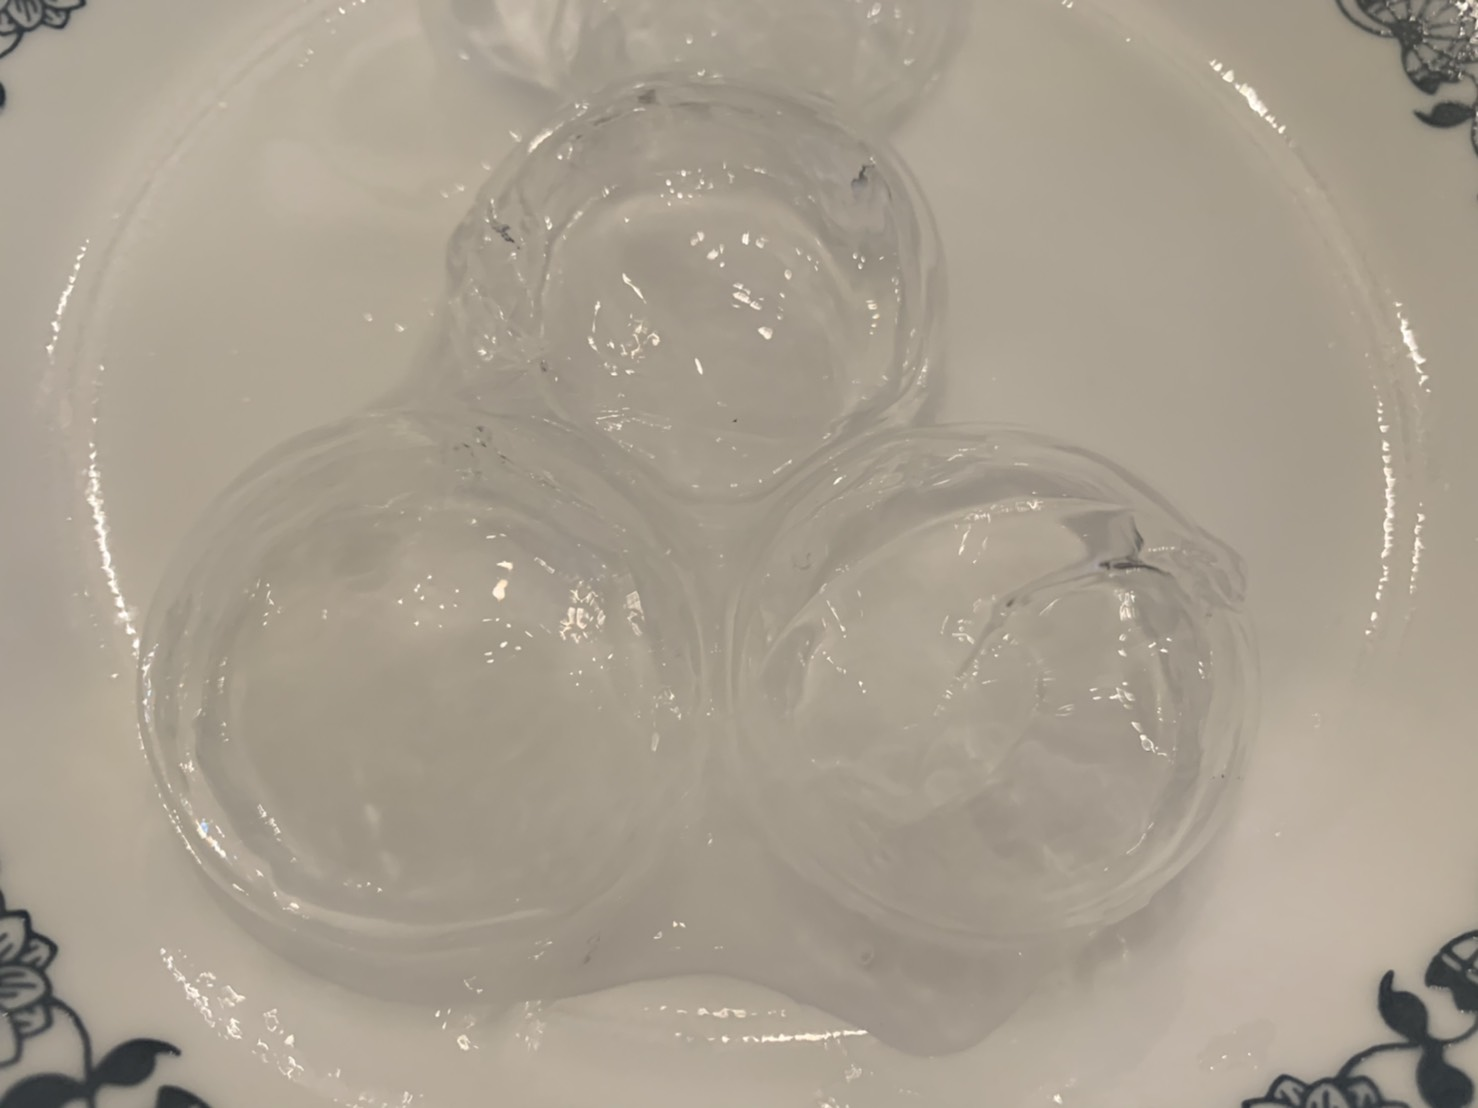
\includegraphics[width = 0.8\columnwidth]{zeri2.jpg}
    \caption{空洞のあるゼリー}
    \label{zeri}
  \end{figure}


\subsection{実験の方法}

本実験では香りを閉じこめた直径 3 センチメートルのゼリーを食べることで,風味を想起させ
ることが出来るかを検討する.香りを想起させるために Vape の香りがわかりやすいリキッド二
つの香りを用意した.なお,口内で香りを充満させ風味を感じさせるために食べる際にゼリーを
口内で割るよう一口で口内に入れてもらう.この時に舌に当たる味ではなく鼻から向ける風味を
感じることができるかを判断してもらう.今回の実験では,作成した嗅覚提示ゼリーの有用性を
調査するとともに,中に入れる香りがどの程度の認知を得るか調査した.


今回実験するにあたって四種類のゼリーを用意した.香料を気化させた空気を注射器で吸い取
り,空洞のゼリーに入れたものを青りんごの Vape リキッド図 5.3 とバニラエッセンス図 5.4 の二
種類用意した.この青りんごの香りを含んだゼリーを 1 のゼリー,バニラの香りを含んだゼリー
を 2 のゼリーとする.


また,香料をゼリーの中に入れ,ゼリー内で気化させ中に香りを充満させる方法で青りんごの
Vape リキッドとバニラエッセンスの二種類用意した. この青りんごの香りを含んだゼリーを 3 の
ゼリーバニラの香りを含んだゼリーを 4 のゼリーとする.
この四種類の香りの入ったゼリーを食してもらい風味の感じ方を調査した.